\scanpage{22}
% Reader B independent complete proposal. Manual literal paths; no compilation or rendering performed.
% Only the final simple equality is a conventional display; the other displayed expressions are labels in the adjoining literal drawing groups.
% BEGIN FIGURE B022-F01; full-scan rectangle [240, 55, 1680, 505]; local origin (240,55).
\figure{\begin{tikzpicture}[x=0.0088cm,y=-0.0088cm,every node/.style={inner sep=0pt,outer sep=0pt,anchor=base west}]
\path[use as bounding box] (0,0) rectangle (1440,450);
\begin{scope}[shift={(-240,-55)}]
\node[font=\small,anchor=base west,inner sep=0pt,outer sep=0pt] at (294,130) {\rlap{\unsure{On|Un} procède par récurrence sur $\operatorname{card} K$,}\phantom{\deleted{\unsure{On|Un} procède par récurrence sur $\operatorname{card} K$,}}};
\node[font=\small,anchor=base west,inner sep=0pt,outer sep=0pt] at (312,179) {\inserted{On note d'abord que}};
\node[font=\small,anchor=base west,inner sep=0pt,outer sep=0pt] at (258,233) {\rlap{pour}\phantom{\deleted{pour}}};
\node[font=\small,anchor=base west,inner sep=0pt,outer sep=0pt] at (432,233) {\rlap{prouver}\phantom{\deleted{prouver}}};
\node[font=\small,anchor=base west,inner sep=0pt,outer sep=0pt] at (713,224) {\rlap{que}\phantom{\deleted{que}}};
% BEGIN B022-G01; observed full-scan box [266, 96, 1570, 238].
% Ownership: The two original opening cancellation rules only; all opening words are owned by T01–T03.
% Role/state: Cancellation geometry; no inferred writing chronology.
\draw[line width=.3pt,line cap=round] (327,110) .. controls (623,101) and (990,100) .. (1234,108) .. controls (1370,109) and (1471,118) .. (1566,126);
\draw[line width=.3pt,line cap=round] (268,226) .. controls (437,211) and (605,211) .. (811,215);
% END B022-G01
% BEGIN B022-M01; observed full-scan box [313, 224, 334, 239].
% Ownership: Short detached slash below pour; the word pour stays in T03.
% Role/state: Shape supported; attachment, role, hand and surface origin remain unresolved.
% Complete reading/state candidates: visible short slash; no character assigned
\node[anchor=base west,inner sep=0pt,outer sep=0pt] at (313,239) {\unsure{%
\begin{tikzpicture}[x=0.0088cm,y=-0.0088cm,baseline=(B),every node/.style={inner sep=0pt,outer sep=0pt,anchor=base west}]
\path[use as bounding box] (0,0) rectangle (21,15);
\coordinate (B) at (0,15);
\begin{scope}[shift={(-313,-224)}]
\draw[line width=.4pt,line cap=round] (318,234) -- (331,228);
\end{scope}
\end{tikzpicture}%
}};
% END B022-M01
\node[font=\normalsize,anchor=base west,inner sep=0pt,outer sep=0pt] at (884,222) {(si};
\node[font=\normalsize,anchor=base west,inner sep=0pt,outer sep=0pt] at (1015,218) {$V=X\setminus$};
% BEGIN B022-G02; observed full-scan box [1153, 166, 1218, 253].
% Ownership: Top union operator and its alpha-in-K lower limit.
% Role/state: The upper-left stem is interrupted before the returning bowl; both runs are preserved.
\draw[line width=.45pt,line cap=round] (1168,175) .. controls (1169,185) and (1170,190) .. (1170,196);
\draw[line width=.45pt,line cap=round] (1171,202) .. controls (1173,216) and (1193,218) .. (1205,204) .. controls (1216,189) and (1209,179) .. (1200,169);
\node[font=\scriptsize,anchor=base west,inner sep=0pt,outer sep=0pt] at (1157,244) {$\alpha\in K$};
% END B022-G02
% BEGIN B022-S01; observed full-scan box [1214, 151, 1293, 231].
% Ownership: Complete Sigma glyph, its head/body, roof, index \alpha and raised +; no adjoining word.
% Role/state: The head and body form the locally observed connected letter shape.
% Complete reading/state candidates: \widehat{\Sigma}_{\alpha}^{+}
\draw[line width=.45pt,line cap=round,line join=round] (1253,183) -- (1223,182) .. controls (1226,189) and (1245,190) .. (1253,197) .. controls (1245,202) and (1230,207) .. (1221,211) -- (1261,212);
\draw[line width=.45pt,line cap=round,line join=round] (1229,167) -- (1251,157) -- (1272,169);
\node[font=\scriptsize,anchor=base west,inner sep=0pt,outer sep=0pt] at (1247,225) {$\alpha$};
\node[font=\scriptsize,anchor=base west,inner sep=0pt,outer sep=0pt] at (1266,191) {$+$};
\node[font=\scriptsize,anchor=base west,inner sep=0pt,outer sep=0pt] at (1214,231) {\phantom{$\widehat{\Sigma}_{\alpha}^{+}$}};
% END B022-S01
\node[font=\small,anchor=base west,inner sep=0pt,outer sep=0pt] at (1304,226) {,};
\node[font=\small,anchor=base west,inner sep=0pt,outer sep=0pt] at (1339,218) {les};
% BEGIN B022-S02; observed full-scan box [1443, 158, 1520, 226].
% Ownership: Complete Sigma glyph, its head/body, roof, index \alpha and raised +; no adjoining word.
% Role/state: The short head and body are separately drawn. The head/independent-rule role remains unresolved; no mathematical operation is assigned to that separation.
% Complete reading/state candidates: \widehat{\Sigma}_{\alpha}^{+} with head stroke | same visible shape with unassigned independent-rule role
\node[anchor=base west,inner sep=0pt,outer sep=0pt] at (1443,226) {\unsure{%
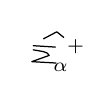
\begin{tikzpicture}[x=0.0088cm,y=-0.0088cm,baseline=(B),every node/.style={inner sep=0pt,outer sep=0pt,anchor=base west}]
\path[use as bounding box] (0,0) rectangle (77,68);
\coordinate (B) at (0,68);
\begin{scope}[shift={(-1443,-158)}]
\draw[line width=.45pt,line cap=round,line join=round] (1451,184) -- (1483,186);
\draw[line width=.45pt,line cap=round,line join=round] (1451,190) .. controls (1461,192) and (1472,192) .. (1474,198) -- (1449,207) -- (1484,209);
\draw[line width=.45pt,line cap=round,line join=round] (1466,174) -- (1485,164) -- (1495,172);
\node[font=\scriptsize,anchor=base west,inner sep=0pt,outer sep=0pt] at (1480,221) {$\alpha$};
\node[font=\scriptsize,anchor=base west,inner sep=0pt,outer sep=0pt] at (1500,193) {$+$};
\node[font=\scriptsize,anchor=base west,inner sep=0pt,outer sep=0pt] at (1443,226) {\phantom{$\widehat{\Sigma}_{\alpha}^{+}$}};
\end{scope}
\end{tikzpicture}%
}};
% END B022-S02
% BEGIN B022-G03; observed full-scan box [1526, 182, 1635, 231].
% Ownership: Opening curve and immediately adjoining alpha-in-K; no second printed alpha is outside this group.
% Role/state: C022-R01 retained: parenthesis primary; attachment as a left lead into alpha remains possible.
% Complete reading/state candidates: (\alpha\in K | \alpha\in K with the same visible left lead
\node[anchor=base west,inner sep=0pt,outer sep=0pt] at (1526,231) {\unsure{%
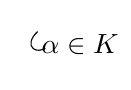
\begin{tikzpicture}[x=0.0088cm,y=-0.0088cm,baseline=(B),every node/.style={inner sep=0pt,outer sep=0pt,anchor=base west}]
\path[use as bounding box] (0,0) rectangle (109,49);
\coordinate (B) at (0,49);
\begin{scope}[shift={(-1526,-182)}]
\draw[line width=.4pt,line cap=round] (1540,188) .. controls (1530,197) and (1528,208) .. (1534,212) .. controls (1539,216) and (1545,215) .. (1551,212);
\node[font=\normalsize,anchor=base west,inner sep=0pt,outer sep=0pt] at (1546,219) {$\alpha\in K$};
\node[font=\scriptsize,anchor=base west,inner sep=0pt,outer sep=0pt] at (1526,231) {\phantom{$\unsure{(}\alpha\in K$}};
\end{scope}
\end{tikzpicture}%
}};
% END B022-G03
\node[font=\scriptsize,anchor=base west,inner sep=0pt,outer sep=0pt] at (1451,272) {étant disjoints};
% BEGIN B022-G04; observed full-scan box [1639, 208, 1678, 301].
% Ownership: Both surviving right-edge closure runs, after the alpha-in-K line and after disjoints.
% Role/state: One spanning close versus two distinct closes is unresolved; the physical edge supplies no connecting ink.
% Complete reading/state candidates: ) | ) )
\node[anchor=base west,inner sep=0pt,outer sep=0pt] at (1639,301) {\unsure{%
\begin{tikzpicture}[x=0.0088cm,y=-0.0088cm,baseline=(B),every node/.style={inner sep=0pt,outer sep=0pt,anchor=base west}]
\path[use as bounding box] (0,0) rectangle (39,93);
\coordinate (B) at (0,93);
\begin{scope}[shift={(-1639,-208)}]
\draw[line width=.3pt,line cap=round] (1662,213) .. controls (1669,219) and (1672,229) .. (1676,240);
\draw[line width=.4pt,line cap=round] (1666,262) .. controls (1662,276) and (1653,287) .. (1644,296);
\node[font=\scriptsize,anchor=base west,inner sep=0pt,outer sep=0pt] at (1639,301) {\phantom{$\unsure{)|)\,)}$}};
\end{scope}
\end{tikzpicture}%
}};
% END B022-G04
% BEGIN B022-G05; observed full-scan box [1077, 250, 1270, 306].
% Ownership: Complete hooked lower bracket and the descending equality strokes; no central brace cusp is supplied.
% Role/state: The bracket attaches the next intersection to X setminus the union.
\draw[line width=.45pt,line cap=round] (1083,255) .. controls (1078,264) and (1079,272) .. (1087,273) .. controls (1137,272) and (1205,276) .. (1251,273) .. controls (1266,273) and (1267,262) .. (1260,261);
\draw[line width=.5pt,line cap=round] (1161,284) -- (1162,299);
\draw[line width=.5pt,line cap=round] (1171,284) -- (1172,301);
% END B022-G05
% BEGIN B022-G06; observed full-scan box [1102, 306, 1166, 385].
% Ownership: Inserted intersection sign and its alpha-in-K lower limit.
% Role/state: Added below the bracket; its formula continues with S03.
\draw[line width=.55pt,line cap=round] (1126,338) .. controls (1120,321) and (1130,312) .. (1141,313) .. controls (1154,311) and (1164,320) .. (1164,337);
\node[font=\scriptsize,anchor=base west,inner sep=0pt,outer sep=0pt] at (1106,379) {$\alpha\in K$};
\node[font=\scriptsize,anchor=base west,inner sep=0pt,outer sep=0pt] at (1102,385) {\phantom{$\inserted{\bigcap_{\alpha\in K}}$}};
% END B022-G06
% BEGIN B022-S03; observed full-scan box [1164, 306, 1245, 356].
% Ownership: Complete Sigma glyph, its head/body, index \alpha and raised -; no adjoining word.
% Role/state: The head and body form the locally observed connected letter shape.
% Complete reading/state candidates: \Sigma_{\alpha}^{-}
\draw[line width=.45pt,line cap=round,line join=round] (1200,314) -- (1172,313) .. controls (1165,315) and (1166,320) .. (1175,321) -- (1195,326) -- (1172,340) -- (1203,341);
\node[font=\scriptsize,anchor=base west,inner sep=0pt,outer sep=0pt] at (1205,352) {$\alpha$};
\node[font=\scriptsize,anchor=base west,inner sep=0pt,outer sep=0pt] at (1213,322) {$-$};
\node[font=\scriptsize,anchor=base west,inner sep=0pt,outer sep=0pt] at (1164,356) {\phantom{$\Sigma_{\alpha}^{-}$}};
% END B022-S03
% BEGIN B022-G07; observed full-scan box [532, 288, 565, 486].
% Ownership: The complete left brace, including its closed middle loop.
% Role/state: The loop and curved lower arm are drawn once beside the two conditions.
\draw[line width=.4pt,line cap=round] (549,294) .. controls (558,334) and (551,370) .. (547,382) .. controls (536,379) and (533,391) .. (540,393) .. controls (548,395) and (551,385) .. (547,382) .. controls (559,396) and (558,431) .. (554,448) .. controls (551,463) and (554,475) .. (559,480);
% END B022-G07
\node[font=\Large,anchor=base west,inner sep=0pt,outer sep=0pt] at (590,340) {$\overline V\cap E_\alpha\ne\varnothing$};
\node[font=\Large,anchor=base west,inner sep=0pt,outer sep=0pt] at (590,455) {$V\cap$};
% BEGIN B022-S04; observed full-scan box [678, 397, 786, 466].
% Ownership: Complete Sigma glyph, its head/body, index \alpha and raised -; no adjoining word.
% Role/state: The short head and body are separately drawn. The head/independent-rule role remains unresolved; no mathematical operation is assigned to that separation.
% Complete reading/state candidates: \Sigma_{\alpha}^{-} with head stroke | same visible shape with unassigned independent-rule role
\draw[line width=.45pt,line cap=round,line join=round] (686,408) -- (726,403);
\draw[line width=.45pt,line cap=round,line join=round] (685,415) .. controls (710,419) and (730,424) .. (727,432) -- (684,452) -- (731,452);
\node[font=\scriptsize,anchor=base west,inner sep=0pt,outer sep=0pt] at (734,459) {$\alpha$};
\node[font=\scriptsize,anchor=base west,inner sep=0pt,outer sep=0pt] at (749,411) {$-$};
\node[font=\scriptsize,anchor=base west,inner sep=0pt,outer sep=0pt] at (678,466) {\phantom{$\Sigma_{\alpha}^{-}$}};
% END B022-S04
% BEGIN B022-G08; observed full-scan box [794, 384, 925, 485].
% Ownership: The old relation and its old empty-set glyph, including their local cancellation strokes; replacement is T10.
% Role/state: C022-R03 retained. The short upright can belong to the relation or to its cancellation; all old ink is retained.
% Complete reading/state candidates: \deleted{\ne\varnothing} | \deleted{=\varnothing}
\node[anchor=base west,inner sep=0pt,outer sep=0pt] at (794,485) {\unsure{%
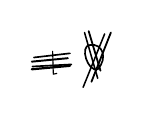
\begin{tikzpicture}[x=0.0088cm,y=-0.0088cm,baseline=(B),every node/.style={inner sep=0pt,outer sep=0pt,anchor=base west}]
\path[use as bounding box] (0,0) rectangle (131,101);
\coordinate (B) at (0,101);
\begin{scope}[shift={(-794,-384)}]
\draw[line width=.6pt,line cap=round] (803,427) -- (855,421);
\draw[line width=.6pt,line cap=round] (801,440) -- (857,437);
\draw[line width=.4pt,line cap=round] (830,418) -- (831,451) -- (836,450);
\draw[line width=.7pt,line cap=round] (800,433) -- (852,428);
\draw[line width=.8pt,line cap=round] (800,444) -- (855,439);
\draw[line width=.6pt,line cap=round] (884,409) .. controls (868,410) and (881,449) .. (895,444) .. controls (910,428) and (902,406) .. (884,409);
\draw[line width=.55pt,line cap=round] (905,393) -- (874,470);
\draw[line width=.55pt,line cap=round] (876,391) -- (895,457);
\draw[line width=.65pt,line cap=round] (882,389) -- (899,446);
\draw[line width=.65pt,line cap=round] (914,391) -- (886,462);
\node[font=\scriptsize,anchor=base west,inner sep=0pt,outer sep=0pt] at (794,485) {\phantom{$\deleted{\unsure{\ne|=}\varnothing}$}};
\end{scope}
\end{tikzpicture}%
}};
% END B022-G08
\node[font=\Large,anchor=base west,inner sep=0pt,outer sep=0pt] at (937,449) {$\ne\varnothing$};
\node[font=\small,anchor=base west,inner sep=0pt,outer sep=0pt] at (1092,441) {alors que};
\node[font=\large,anchor=base west,inner sep=0pt,outer sep=0pt] at (1340,443) {$V\cap$};
% BEGIN B022-S05; observed full-scan box [1409, 392, 1491, 450].
% Ownership: Complete Sigma glyph, its head/body, index \alpha and raised +; no adjoining word.
% Role/state: The head and body form the locally observed connected letter shape.
% Complete reading/state candidates: \Sigma_{\alpha}^{+}
\draw[line width=.45pt,line cap=round,line join=round] (1447,402) -- (1416,402) .. controls (1412,405) and (1419,409) .. (1436,411) .. controls (1450,416) and (1430,426) .. (1415,431) -- (1447,432);
\node[font=\scriptsize,anchor=base west,inner sep=0pt,outer sep=0pt] at (1450,445) {$\alpha$};
\node[font=\scriptsize,anchor=base west,inner sep=0pt,outer sep=0pt] at (1464,407) {$+$};
\node[font=\scriptsize,anchor=base west,inner sep=0pt,outer sep=0pt] at (1409,450) {\phantom{$\Sigma_{\alpha}^{+}$}};
% END B022-S05
\node[font=\large,anchor=base west,inner sep=0pt,outer sep=0pt] at (1504,442) {$=\varnothing$};
\node[font=\scriptsize,anchor=base west,inner sep=0pt,outer sep=0pt] at (410,454) {trivial};
% BEGIN B022-G09; observed full-scan box [470, 427, 587, 452].
% Ownership: The arrow from the marginal word trivial to the second condition. The word itself belongs to T14.
% Role/state: Arrow crosses the brace and ends before the V.
\draw[line width=.3pt,line cap=round] (474,447) -- (580,435);
\draw[line width=.5pt,line cap=round] (574,431) -- (582,435) -- (575,439);
% END B022-G09
\end{scope}
\end{tikzpicture}}
% END FIGURE B022-F01

De façon précise, je dis que

% BEGIN FIGURE B022-F02; full-scan rectangle [240, 630, 1678, 1938]; local origin (240,630).
\figure{\begin{tikzpicture}[x=0.0088cm,y=-0.0088cm,every node/.style={inner sep=0pt,outer sep=0pt,anchor=base west}]
\path[use as bounding box] (0,0) rectangle (1438,1308);
\begin{scope}[shift={(-240,-630)}]
\node[font=\Large,anchor=base west,inner sep=0pt,outer sep=0pt] at (608,730) {$\overline V\cap E_\alpha=$};
% BEGIN B022-S06; observed full-scan box [905, 640, 1023, 735].
% Ownership: Complete Sigma glyph, its head/body, outer bar, index \alpha and raised -; no adjoining word.
% Role/state: The head and body form the locally observed connected letter shape.
% Complete reading/state candidates: \overline{\Sigma_{\alpha}^{-}}
\draw[line width=.45pt,line cap=round,line join=round] (966,668) -- (917,667) -- (945,689) -- (913,716) -- (965,714);
\draw[line width=.45pt,line cap=round] (920,651) .. controls (942,647) and (975,647) .. (995,650);
\node[font=\scriptsize,anchor=base west,inner sep=0pt,outer sep=0pt] at (968,725) {$\alpha$};
\node[font=\scriptsize,anchor=base west,inner sep=0pt,outer sep=0pt] at (984,678) {$-$};
\node[font=\scriptsize,anchor=base west,inner sep=0pt,outer sep=0pt] at (905,735) {\phantom{$\overline{\Sigma_{\alpha}^{-}}$}};
% END B022-S06
\node[font=\Large,anchor=base west,inner sep=0pt,outer sep=0pt] at (1040,723) {$\cap E_\alpha$};
\node[font=\small,anchor=base west,inner sep=0pt,outer sep=0pt] at (1253,711) {(qui est donc $\ne\varnothing$)};
% BEGIN B022-G10; observed full-scan box [680, 744, 713, 779].
% Ownership: The two descending equality strokes below the main left member.
% Role/state: Both strokes are clear; they precede the qualified lower left annotation.
\draw[line width=.4pt,line cap=round] (687,750) -- (695,764);
\draw[line width=.4pt,line cap=round] (699,752) -- (707,771);
% END B022-G10
% BEGIN B022-G11; observed full-scan box [722, 741, 877, 817].
% Ownership: Complete lower left annotation: V with bar, cap, hatted Sigma S07 with its separate head, alpha and plus.
% Role/state: Primary deleted by the shared long line G14-C1; live annotation remains an alternative. The head/independent-rule role is also locally retained under the recurring sign convention.
% Complete reading/state candidates: \deleted{\overline V\cap\widehat{\Sigma}_\alpha^+} | \overline V\cap\widehat{\Sigma}_\alpha^+
\node[anchor=base west,inner sep=0pt,outer sep=0pt] at (722,817) {\unsure{%
\begin{tikzpicture}[x=0.0088cm,y=-0.0088cm,baseline=(B),every node/.style={inner sep=0pt,outer sep=0pt,anchor=base west}]
\path[use as bounding box] (0,0) rectangle (155,76);
\coordinate (B) at (0,76);
\begin{scope}[shift={(-722,-741)}]
\node[font=\scriptsize,anchor=base west,inner sep=0pt,outer sep=0pt] at (725,804) {$\overline V\cap$};
\draw[line width=.4pt,line cap=round] (808,772) -- (841,768);
\draw[line width=.4pt,line cap=round] (806,778) -- (827,782) -- (805,791) -- (841,790);
\draw[line width=.4pt,line cap=round] (816,758) -- (835,747) -- (849,756);
\node[font=\scriptsize,anchor=base west,inner sep=0pt,outer sep=0pt] at (839,796) {$\alpha$};
\node[font=\scriptsize,anchor=base west,inner sep=0pt,outer sep=0pt] at (850,776) {$+$};
\node[font=\scriptsize,anchor=base west,inner sep=0pt,outer sep=0pt] at (722,814) {\phantom{$\unsure{\deleted{\overline V\cap\widehat{\Sigma}_\alpha^+}|\overline V\cap\widehat{\Sigma}_\alpha^+}$}};
\end{scope}
\end{tikzpicture}%
}};
% END B022-G11
% BEGIN B022-G12; observed full-scan box [1000, 726, 1190, 803].
% Ownership: Complete lower right formula: Sigma S08 with separate head, minus and alpha; cap; hatted Sigma S09 with alpha and plus. Its shared upper run is exclusively G13.
% Role/state: Primary deleted by the same G14-C1 line; live annotation remains an alternative. No ordinary overline duplicates the horizontal G13 run.
% Complete reading/state candidates: \deleted{\overline{\Sigma_\alpha^-}\cap\widehat{\Sigma}_\alpha^+} | \overline{\Sigma_\alpha^-}\cap\widehat{\Sigma}_\alpha^+
\node[anchor=base west,inner sep=0pt,outer sep=0pt] at (1000,803) {\unsure{%
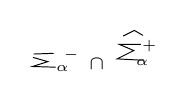
\begin{tikzpicture}[x=0.0088cm,y=-0.0088cm,baseline=(B),every node/.style={inner sep=0pt,outer sep=0pt,anchor=base west}]
\path[use as bounding box] (0,0) rectangle (190,77);
\coordinate (B) at (0,77);
\begin{scope}[shift={(-1000,-726)}]
\draw[line width=.35pt,line cap=round] (1009,764) -- (1037,763);
\draw[line width=.35pt,line cap=round] (1008,769) -- (1029,775) -- (1007,782) -- (1040,783);
\node[font=\tiny,anchor=base west,inner sep=0pt,outer sep=0pt] at (1041,789) {$\alpha$};
\node[font=\tiny,anchor=base west,inner sep=0pt,outer sep=0pt] at (1052,771) {$-$};
\node[font=\scriptsize,anchor=base west,inner sep=0pt,outer sep=0pt] at (1089,786) {$\cap$};
\draw[line width=.35pt,line cap=round] (1163,750) -- (1132,750) -- (1153,759) -- (1129,771) -- (1166,773);
\draw[line width=.35pt,line cap=round] (1138,738) -- (1154,730) -- (1166,737);
\node[font=\tiny,anchor=base west,inner sep=0pt,outer sep=0pt] at (1156,780) {$\alpha$};
\node[font=\tiny,anchor=base west,inner sep=0pt,outer sep=0pt] at (1165,757) {$+$};
\node[font=\scriptsize,anchor=base west,inner sep=0pt,outer sep=0pt] at (1000,799) {\phantom{$\unsure{\deleted{\overline{\Sigma_\alpha^-}\cap\widehat{\Sigma}_\alpha^+}|\overline{\Sigma_\alpha^-}\cap\widehat{\Sigma}_\alpha^+}$}};
\end{scope}
\end{tikzpicture}%
}};
% END B022-G12
% BEGIN B022-G13; observed full-scan box [1005, 731, 1077, 759].
% Ownership: The complete short horizontal run and three crossing/raised slants over S08; no second closure rule or generic connector is drawn.
% Role/state: C022-R04 retained: crossed descending equality primary, live equality and arrow-like interpretation remain; the apportionment between connector and formula bar is unresolved.
% Complete reading/state candidates: \rotatebox{90}{$\deleted{=}$} | \rotatebox{90}{$=$} | \rotatebox{90}{$\Rightarrow$}
\node[anchor=base west,inner sep=0pt,outer sep=0pt] at (1005,759) {\unsure{%
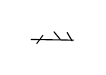
\begin{tikzpicture}[x=0.0088cm,y=-0.0088cm,baseline=(B),every node/.style={inner sep=0pt,outer sep=0pt,anchor=base west}]
\path[use as bounding box] (0,0) rectangle (72,28);
\coordinate (B) at (0,28);
\begin{scope}[shift={(-1005,-731)}]
\draw[line width=.4pt,line cap=round] (1010,748) -- (1071,749);
\draw[line width=.35pt,line cap=round] (1018,754) -- (1027,742);
\draw[line width=.4pt,line cap=round] (1043,737) -- (1052,748);
\draw[line width=.4pt,line cap=round] (1062,738) -- (1069,750);
\node[font=\scriptsize,anchor=base west,inner sep=0pt,outer sep=0pt] at (1005,759) {\phantom{$\rotatebox{90}{$\unsure{\deleted{=}|=|\Rightarrow}$}$}};
\end{scope}
\end{tikzpicture}%
}};
% END B022-G13
\node[font=\small,anchor=base west,inner sep=0pt,outer sep=0pt] at (263,852) {\rlap{Comme}\phantom{\deleted{Comme}}};
\node[font=\large,anchor=base west,inner sep=0pt,outer sep=0pt] at (618,850) {\rlap{$V\subset$}\phantom{\deleted{$V\subset$}}};
% BEGIN B022-S10; observed full-scan box [735, 798, 830, 859].
% Ownership: Complete Sigma glyph, its head/body, index \alpha and raised -; no adjoining word.
% Role/state: The head and body form the locally observed connected letter shape.
% Complete reading/state candidates: \Sigma_{\alpha}^{-}
\draw[line width=.45pt,line cap=round,line join=round] (789,806) -- (747,804) -- (771,821) -- (741,845) -- (794,844);
\node[font=\scriptsize,anchor=base west,inner sep=0pt,outer sep=0pt] at (795,854) {$\alpha$};
\node[font=\scriptsize,anchor=base west,inner sep=0pt,outer sep=0pt] at (804,810) {$-$};
\node[font=\scriptsize,anchor=base west,inner sep=0pt,outer sep=0pt] at (735,859) {\phantom{$\deleted{\Sigma_{\alpha}^{-}}$}};
% END B022-S10
\node[font=\small,anchor=base west,inner sep=0pt,outer sep=0pt] at (880,850) {\rlap{, on a}\phantom{\deleted{, on a}}};
\node[font=\large,anchor=base west,inner sep=0pt,outer sep=0pt] at (1167,846) {\rlap{$V\cap E_\alpha\subset$}\phantom{\deleted{$V\cap E_\alpha\subset$}}};
% BEGIN B022-S11; observed full-scan box [1394, 765, 1510, 853].
% Ownership: Complete Sigma glyph, its head/body, outer bar, index \alpha and raised -; no adjoining word.
% Role/state: The short head and body are separately drawn. The head/independent-rule role remains unresolved; no mathematical operation is assigned to that separation.
% Complete reading/state candidates: \overline{\Sigma_{\alpha}^{-}} with head stroke | same visible shape with unassigned independent-rule role
\draw[line width=.45pt,line cap=round,line join=round] (1405,794) -- (1446,791);
\draw[line width=.45pt,line cap=round,line join=round] (1405,800) -- (1436,811) -- (1401,827) -- (1468,826);
\draw[line width=.45pt,line cap=round] (1412,775) -- (1492,771);
\node[font=\scriptsize,anchor=base west,inner sep=0pt,outer sep=0pt] at (1446,843) {$\alpha$};
\node[font=\scriptsize,anchor=base west,inner sep=0pt,outer sep=0pt] at (1459,794) {$-$};
\node[font=\scriptsize,anchor=base west,inner sep=0pt,outer sep=0pt] at (1394,853) {\phantom{$\deleted{\overline{\Sigma_{\alpha}^{-}}}$}};
% END B022-S11
\node[font=\large,anchor=base west,inner sep=0pt,outer sep=0pt] at (1518,846) {\rlap{$\cap E_\alpha$,}\phantom{\deleted{$\cap E_\alpha$,}}};
\node[font=\small,anchor=base west,inner sep=0pt,outer sep=0pt] at (275,983) {\rlap{prouvons}\phantom{\deleted{prouvons}}};
\node[font=\small,anchor=base west,inner sep=0pt,outer sep=0pt] at (576,960) {\rlap{l'inclusion}\phantom{\deleted{l'inclusion}}};
\node[font=\small,anchor=base west,inner sep=0pt,outer sep=0pt] at (936,953) {\rlap{inverse}\phantom{\deleted{inverse}}};
% BEGIN B022-S12; observed full-scan box [557, 1019, 676, 1098].
% Ownership: Complete Sigma glyph, its head/body, outer bar, index \alpha and raised -; no adjoining word.
% Role/state: The head and body form the locally observed connected letter shape.
% Complete reading/state candidates: \overline{\Sigma_{\alpha}^{-}}
\draw[line width=.45pt,line cap=round,line join=round] (621,1047) -- (567,1051) .. controls (565,1055) and (594,1055) .. (610,1062) -- (570,1086) -- (635,1075);
\draw[line width=.45pt,line cap=round] (574,1031) .. controls (603,1031) and (631,1027) .. (665,1026);
\node[font=\scriptsize,anchor=base west,inner sep=0pt,outer sep=0pt] at (621,1092) {$\alpha$};
\node[font=\scriptsize,anchor=base west,inner sep=0pt,outer sep=0pt] at (648,1057) {$-$};
\node[font=\scriptsize,anchor=base west,inner sep=0pt,outer sep=0pt] at (557,1098) {\phantom{$\deleted{\overline{\Sigma_{\alpha}^{-}}}$}};
% END B022-S12
\node[font=\large,anchor=base west,inner sep=0pt,outer sep=0pt] at (680,1089) {\rlap{$\cap E_\alpha\subset\overline V\cap E_\alpha$}\phantom{\deleted{$\cap E_\alpha\subset\overline V\cap E_\alpha$}}};
\node[font=\small,anchor=base west,inner sep=0pt,outer sep=0pt] at (286,1211) {\rlap{Soit}\phantom{\deleted{Soit}}};
\node[font=\large,anchor=base west,inner sep=0pt,outer sep=0pt] at (485,1205) {\rlap{$x\in$}\phantom{\deleted{$x\in$}}};
% BEGIN B022-S13; observed full-scan box [587, 1135, 684, 1213].
% Ownership: Complete Sigma glyph, its head/body, outer bar, index \alpha and raised -; no adjoining word.
% Role/state: The short head and body are separately drawn. The head/independent-rule role remains unresolved; no mathematical operation is assigned to that separation.
% Complete reading/state candidates: \overline{\Sigma_{\alpha}^{-}} with head stroke | same visible shape with unassigned independent-rule role
\draw[line width=.45pt,line cap=round,line join=round] (598,1159) -- (636,1156);
\draw[line width=.45pt,line cap=round,line join=round] (597,1166) -- (624,1174) -- (596,1192) -- (641,1192);
\draw[line width=.45pt,line cap=round] (601,1146) -- (668,1141);
\node[font=\scriptsize,anchor=base west,inner sep=0pt,outer sep=0pt] at (630,1208) {$\alpha$};
\node[font=\scriptsize,anchor=base west,inner sep=0pt,outer sep=0pt] at (647,1162) {$-$};
\node[font=\scriptsize,anchor=base west,inner sep=0pt,outer sep=0pt] at (587,1213) {\phantom{$\deleted{\overline{\Sigma_{\alpha}^{-}}}$}};
% END B022-S13
\node[font=\large,anchor=base west,inner sep=0pt,outer sep=0pt] at (676,1204) {\rlap{$\cap E_\alpha$,}\phantom{\deleted{$\cap E_\alpha$,}}};
\node[font=\small,anchor=base west,inner sep=0pt,outer sep=0pt] at (869,1198) {\rlap{prouvons}\phantom{\deleted{prouvons}}};
\node[font=\large,anchor=base west,inner sep=0pt,outer sep=0pt] at (1164,1193) {\rlap{$x\in\overline V\cap E_\alpha$}\phantom{\deleted{$x\in\overline V\cap E_\alpha$}}};
\node[font=\small,anchor=base west,inner sep=0pt,outer sep=0pt] at (1462,1192) {\rlap{i.e.}\phantom{\deleted{i.e.}}};
\node[font=\large,anchor=base west,inner sep=0pt,outer sep=0pt] at (260,1304) {\rlap{$x\in\overline V$,}\phantom{\deleted{$x\in\overline V$,}}};
\node[font=\small,anchor=base west,inner sep=0pt,outer sep=0pt] at (493,1303) {\rlap{soit}\phantom{\deleted{soit}}};
\node[font=\large,anchor=base west,inner sep=0pt,outer sep=0pt] at (657,1292) {\rlap{$W$}\phantom{\deleted{$W$}}};
\node[font=\small,anchor=base west,inner sep=0pt,outer sep=0pt] at (713,1292) {\rlap{un}\phantom{\deleted{un}}};
\node[font=\small,anchor=base west,inner sep=0pt,outer sep=0pt] at (820,1293) {\rlap{voisinage}\phantom{\deleted{voisinage}}};
\node[font=\small,anchor=base west,inner sep=0pt,outer sep=0pt] at (1066,1285) {\rlap{de}\phantom{\deleted{de}}};
\node[font=\large,anchor=base west,inner sep=0pt,outer sep=0pt] at (1156,1285) {\rlap{$x$,}\phantom{\deleted{$x$,}}};
\node[font=\small,anchor=base west,inner sep=0pt,outer sep=0pt] at (1250,1277) {\rlap{montrons qu'il}\phantom{\deleted{montrons qu'il}}};
\node[font=\small,anchor=base west,inner sep=0pt,outer sep=0pt] at (275,1405) {\rlap{rencontre}\phantom{\deleted{rencontre}}};
\node[font=\small,anchor=base west,inner sep=0pt,outer sep=0pt] at (700,1376) {\rlap{Or}\phantom{\deleted{Or}}};
\node[font=\small,anchor=base west,inner sep=0pt,outer sep=0pt] at (823,1372) {\rlap{\unsure{on}}\phantom{\deleted{\unsure{on}}}};
\node[font=\small,anchor=base west,inner sep=0pt,outer sep=0pt] at (950,1370) {\rlap{peut}\phantom{\deleted{peut}}};
\node[font=\small,anchor=base west,inner sep=0pt,outer sep=0pt] at (1090,1371) {\rlap{considérer}\phantom{\deleted{considérer}}};
\node[font=\small,anchor=base west,inner sep=0pt,outer sep=0pt] at (1460,1385) {\rlap{cette}\phantom{\deleted{cette}}};
\node[font=\small,anchor=base west,inner sep=0pt,outer sep=0pt] at (280,1505) {\rlap{\unsure{formule|relation}}\phantom{\deleted{\unsure{formule|relation}}}};
\node[font=\small,anchor=base west,inner sep=0pt,outer sep=0pt] at (333,1464) {\rlap{\inserted{égalité}}\phantom{\deleted{\inserted{égalité}}}};
\node[font=\small,anchor=base west,inner sep=0pt,outer sep=0pt] at (566,1486) {\rlap{comme}\phantom{\deleted{comme}}};
\node[font=\small,anchor=base west,inner sep=0pt,outer sep=0pt] at (891,1484) {\rlap{\unsure{égalité|egalité}}\phantom{\deleted{\unsure{égalité|egalité}}}};
\node[font=\small,anchor=base west,inner sep=0pt,outer sep=0pt] at (1146,1477) {\rlap{dans}\phantom{\deleted{dans}}};
\node[font=\small,anchor=base west,inner sep=0pt,outer sep=0pt] at (312,1601) {\rlap{l'espace}\phantom{\deleted{l'espace}}};
% BEGIN B022-G15; observed full-scan box [573, 1564, 637, 1636].
% Ownership: The complete old variable before the first equals; no additional generic Y, Z or X is printed.
% Role/state: C022-R07 retained with X added as a supported alternative; all strokes are preserved without assigning each stroke to letter or local cancellation.
% Complete reading/state candidates: \deleted{Y} | \deleted{Z} | \deleted{X}
\node[anchor=base west,inner sep=0pt,outer sep=0pt] at (573,1636) {\unsure{%
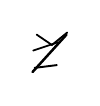
\begin{tikzpicture}[x=0.0088cm,y=-0.0088cm,baseline=(B),every node/.style={inner sep=0pt,outer sep=0pt,anchor=base west}]
\path[use as bounding box] (0,0) rectangle (64,72);
\coordinate (B) at (0,72);
\begin{scope}[shift={(-573,-1564)}]
\draw[line width=.65pt,line cap=round] (586,1574) -- (608,1589) -- (630,1571);
\draw[line width=.9pt,line cap=round] (629,1574) -- (580,1628);
\draw[line width=.7pt,line cap=round] (583,1622) -- (615,1618);
\draw[line width=.65pt,line cap=round] (581,1597) -- (617,1585);
\node[font=\scriptsize,anchor=base west,inner sep=0pt,outer sep=0pt] at (573,1636) {\phantom{$\deleted{\unsure{Y|Z|X}}$}};
\end{scope}
\end{tikzpicture}%
}};
% END B022-G15
\node[font=\large,anchor=base west,inner sep=0pt,outer sep=0pt] at (641,1615) {\rlap{$=$}\phantom{\deleted{$=$}}};
% BEGIN B022-S14; observed full-scan box [718, 1538, 831, 1624].
% Ownership: Complete Sigma glyph, its head/body, roof, index \alpha and raised -; no adjoining word.
% Role/state: The short head and body are separately drawn. The head/independent-rule role remains unresolved; no mathematical operation is assigned to that separation.
% Complete reading/state candidates: \widehat{\Sigma}_{\alpha}^{-} with head stroke | same visible shape with unassigned independent-rule role
\draw[line width=.45pt,line cap=round,line join=round] (726,1581) -- (773,1580);
\draw[line width=.45pt,line cap=round,line join=round] (725,1587) -- (754,1596) -- (723,1613) -- (778,1611);
\draw[line width=.45pt,line cap=round,line join=round] (759,1551) -- (784,1540) -- (802,1552);
\node[font=\scriptsize,anchor=base west,inner sep=0pt,outer sep=0pt] at (785,1620) {$\alpha$};
\node[font=\scriptsize,anchor=base west,inner sep=0pt,outer sep=0pt] at (800,1585) {$-$};
\node[font=\scriptsize,anchor=base west,inner sep=0pt,outer sep=0pt] at (718,1624) {\phantom{$\deleted{\widehat{\Sigma}_{\alpha}^{-}}$}};
% END B022-S14
\node[font=\large,anchor=base west,inner sep=0pt,outer sep=0pt] at (847,1609) {\rlap{$=$}\phantom{\deleted{$=$}}};
% BEGIN B022-S15; observed full-scan box [893, 1575, 982, 1626].
% Ownership: Complete Sigma glyph, its head/body, index \alpha and raised -; no adjoining word.
% Role/state: The short head and body are separately drawn. The head/independent-rule role remains unresolved; no mathematical operation is assigned to that separation.
% Complete reading/state candidates: \Sigma_{\alpha}^{-} with head stroke | same visible shape with unassigned independent-rule role
\draw[line width=.45pt,line cap=round,line join=round] (900,1582) -- (934,1580);
\draw[line width=.45pt,line cap=round,line join=round] (900,1588) -- (927,1596) -- (898,1609) -- (939,1609);
\node[font=\scriptsize,anchor=base west,inner sep=0pt,outer sep=0pt] at (938,1620) {$\alpha$};
\node[font=\scriptsize,anchor=base west,inner sep=0pt,outer sep=0pt] at (954,1591) {$-$};
\node[font=\scriptsize,anchor=base west,inner sep=0pt,outer sep=0pt] at (893,1626) {\phantom{$\deleted{\Sigma_{\alpha}^{-}}$}};
% END B022-S15
\node[font=\large,anchor=base west,inner sep=0pt,outer sep=0pt] at (1002,1616) {\rlap{$\cup E_\alpha$}\phantom{\deleted{$\cup E_\alpha$}}};
\node[font=\small,anchor=base west,inner sep=0pt,outer sep=0pt] at (306,1734) {\rlap{dans}\phantom{\deleted{dans}}};
\node[font=\small,anchor=base west,inner sep=0pt,outer sep=0pt] at (463,1722) {\rlap{lequel}\phantom{\deleted{lequel}}};
\node[font=\small,anchor=base west,inner sep=0pt,outer sep=0pt] at (747,1712) {\rlap{on a}\phantom{\deleted{on a}}};
\node[font=\small,anchor=base west,inner sep=0pt,outer sep=0pt] at (947,1705) {\rlap{deux}\phantom{\deleted{deux}}};
\node[font=\small,anchor=base west,inner sep=0pt,outer sep=0pt] at (1095,1708) {\rlap{parties}\phantom{\deleted{parties}}};
\node[font=\small,anchor=base west,inner sep=0pt,outer sep=0pt] at (1295,1706) {\rlap{fermées}\phantom{\deleted{fermées}}};
\node[font=\small,anchor=base west,inner sep=0pt,outer sep=0pt] at (300,1842) {\rlap{disjointes}\phantom{\deleted{disjointes}}};
% BEGIN B022-G14; observed full-scan box [263, 765, 1606, 1856].
% Ownership: All connected frame/cancellation runs C1–C14. C1 also passes through the feet of the two small lower annotations. All words and formula glyphs are owned separately; no text is embedded in these paths.
% Role/state: The passage is deleted. Path 11 and 12 preserve the lower left interruption. No generic visible sout stroke is added.
\draw[line width=.4pt,line cap=round] (267,835) .. controls (505,826) and (697,801) .. (912,789) .. controls (1178,775) and (1455,767) .. (1578,777);
\draw[line width=.3pt,line cap=round] (281,838) .. controls (294,936) and (298,1095) .. (309,1210) .. controls (310,1292) and (304,1352) .. (283,1394);
\draw[line width=.35pt,line cap=round] (276,1394) .. controls (391,1408) and (520,1394) .. (638,1383) .. controls (623,1344) and (614,1305) .. (651,1285) .. controls (866,1285) and (1138,1290) .. (1328,1284) .. controls (1335,1284) and (1338,1281) .. (1331,1277);
\draw[line width=.4pt,line cap=round] (282,1402) -- (283,1497) .. controls (284,1528) and (332,1520) .. (403,1512) .. controls (658,1484) and (979,1473) .. (1279,1466) .. controls (1428,1475) and (1485,1450) .. (1524,1393) .. controls (1551,1352) and (1569,1333) .. (1600,1316);
\draw[line width=.35pt,line cap=round] (311,1512) -- (312,1597) .. controls (314,1630) and (382,1633) .. (493,1621) .. controls (613,1606) and (672,1583) .. (777,1592) .. controls (977,1602) and (1117,1621) .. (1225,1600) .. controls (1287,1589) and (1329,1558) .. (1346,1543);
\draw[line width=.3pt,line cap=round] (515,845) .. controls (574,946) and (632,1068) .. (704,1190) .. controls (740,1245) and (774,1282) .. (812,1288);
\draw[line width=.3pt,line cap=round] (986,895) .. controls (1043,1016) and (1107,1176) .. (1169,1298) .. controls (1197,1351) and (1225,1394) .. (1244,1412);
\draw[line width=.35pt,line cap=round] (815,1324) .. controls (857,1374) and (896,1438) .. (950,1472);
\draw[line width=.3pt,line cap=round] (1394,845) .. controls (1445,953) and (1490,1086) .. (1507,1142);
\draw[line width=.4pt,line cap=round] (308,1735) .. controls (666,1718) and (1080,1701) .. (1516,1710);
\draw[line width=.3pt,line cap=round] (308,1736) .. controls (302,1762) and (298,1787) .. (296,1804);
\draw[line width=.35pt,line cap=round] (296,1809) .. controls (294,1839) and (330,1848) .. (377,1840) .. controls (467,1832) and (540,1828) .. (590,1823) .. controls (638,1820) and (648,1810) .. (627,1745);
\draw[line width=.65pt,line cap=round] (821,1364) .. controls (847,1355) and (886,1364) .. (917,1368);
\draw[line width=.6pt,line cap=round] (276,1500) .. controls (349,1490) and (431,1494) .. (494,1494);
% END B022-G14
% BEGIN B022-M02; observed full-scan box [245, 885, 257, 904].
% Ownership: Tiny curved stroke left of the cancellation frame; no adjoining word.
% Role/state: Shape supported; role, hand and surface origin remain unresolved.
% Complete reading/state candidates: small curved stroke; no character assigned
\node[anchor=base west,inner sep=0pt,outer sep=0pt] at (245,904) {\unsure{%
\begin{tikzpicture}[x=0.0088cm,y=-0.0088cm,baseline=(B),every node/.style={inner sep=0pt,outer sep=0pt,anchor=base west}]
\path[use as bounding box] (0,0) rectangle (12,19);
\coordinate (B) at (0,19);
\begin{scope}[shift={(-245,-885)}]
\draw[line width=.3pt,line cap=round] (253,890) .. controls (250,893) and (249,897) .. (251,900);
\end{scope}
\end{tikzpicture}%
}};
% END B022-M02
% BEGIN B022-M06; observed full-scan box [302, 1507, 312, 1517].
% Ownership: Small point below the beginning of the old noun; noun itself belongs to T32.
% Role/state: The point may attach to the noun or its cancellation; its role and hand remain unresolved. No letter is supplied from it.
% Complete reading/state candidates: point; attachment unresolved
\node[anchor=base west,inner sep=0pt,outer sep=0pt] at (302,1517) {\unsure{%
\begin{tikzpicture}[x=0.0088cm,y=-0.0088cm,baseline=(B),every node/.style={inner sep=0pt,outer sep=0pt,anchor=base west}]
\path[use as bounding box] (0,0) rectangle (10,10);
\coordinate (B) at (0,10);
\begin{scope}[shift={(-302,-1507)}]
\fill (307,1512) circle[radius=1.2];
\end{scope}
\end{tikzpicture}%
}};
% END B022-M06
% BEGIN B022-M07; observed full-scan box [1649, 1725, 1665, 1743].
% Ownership: Two separate small points near the right paper edge, beside the lower cancelled/live transition; no adjoining word.
% Role/state: Both shapes are supported; attachment, role, hand and surface origin remain unresolved.
% Complete reading/state candidates: two small points; no punctuation assigned
\node[anchor=base west,inner sep=0pt,outer sep=0pt] at (1649,1743) {\unsure{%
\begin{tikzpicture}[x=0.0088cm,y=-0.0088cm,baseline=(B),every node/.style={inner sep=0pt,outer sep=0pt,anchor=base west}]
\path[use as bounding box] (0,0) rectangle (16,18);
\coordinate (B) at (0,18);
\begin{scope}[shift={(-1649,-1725)}]
\fill (1658.1,1729.3) .. controls (1659.1,1728.3) and (1661.0,1729.1) .. (1660.8,1730.5) .. controls (1660.5,1732.0) and (1658.2,1732.3) .. (1657.7,1731.0) -- cycle;
\fill (1653.0,1736.2) .. controls (1654.2,1735.5) and (1655.9,1736.2) .. (1655.7,1737.7) .. controls (1655.1,1739.0) and (1652.9,1738.8) .. (1652.8,1737.2) -- cycle;
\end{scope}
\end{tikzpicture}%
}};
% END B022-M07
\node[font=\small,anchor=base west,inner sep=0pt,outer sep=0pt] at (717,1792) {Or};
\node[font=\small,anchor=base west,inner sep=0pt,outer sep=0pt] at (824,1782) {dans};
\node[font=\large,anchor=base west,inner sep=0pt,outer sep=0pt] at (1002,1785) {$X$};
\node[font=\small,anchor=base west,inner sep=0pt,outer sep=0pt] at (1058,1785) {on a};
\node[font=\small,anchor=base west,inner sep=0pt,outer sep=0pt] at (1287,1784) {les};
\node[font=\small,anchor=base west,inner sep=0pt,outer sep=0pt] at (1403,1782) {deux};
\node[font=\small,anchor=base west,inner sep=0pt,outer sep=0pt] at (306,1929) {parties};
\node[font=\small,anchor=base west,inner sep=0pt,outer sep=0pt] at (550,1907) {\rlap{fermées}\phantom{\uline{fermées}}};
\node[font=\small,anchor=base west,inner sep=0pt,outer sep=0pt] at (836,1885) {\rlap{disjointes}\phantom{\uline{disjointes}}};
% BEGIN B022-G16; observed full-scan box [625, 1895, 1110, 1931].
% Ownership: The two separate underline strokes beneath fermées and disjointes; words belong to T43 and T44.
% Role/state: Literal spans are retained; no linguistic restriction of emphasis to a partial word is inferred.
\draw[line width=.4pt,line cap=round] (630,1925) -- (757,1916);
\draw[line width=.4pt,line cap=round] (873,1906) -- (1102,1900);
% END B022-G16
% BEGIN B022-M03; observed full-scan box [1210, 1828, 1245, 1859].
% Ownership: Detached oblique stroke above-right of disjointes; no word owned.
% Role/state: Shape high confidence; role, hand, attachment and surface origin unresolved.
% Complete reading/state candidates: short oblique stroke; no character assigned
\node[anchor=base west,inner sep=0pt,outer sep=0pt] at (1210,1859) {\unsure{%
\begin{tikzpicture}[x=0.0088cm,y=-0.0088cm,baseline=(B),every node/.style={inner sep=0pt,outer sep=0pt,anchor=base west}]
\path[use as bounding box] (0,0) rectangle (35,31);
\coordinate (B) at (0,31);
\begin{scope}[shift={(-1210,-1828)}]
\draw[line width=.45pt,line cap=round] (1218,1835) -- (1238,1852);
\end{scope}
\end{tikzpicture}%
}};
% END B022-M03
\end{scope}
\end{tikzpicture}}
% END FIGURE B022-F02

% BEGIN FIGURE B022-F03; full-scan rectangle [620, 1928, 1312, 2088]; local origin (620,1928).
\figure{\begin{tikzpicture}[x=0.0088cm,y=-0.0088cm,every node/.style={inner sep=0pt,outer sep=0pt,anchor=base west}]
\path[use as bounding box] (0,0) rectangle (692,160);
\begin{scope}[shift={(-620,-1928)}]
\node[font=\Large,anchor=base west,inner sep=0pt,outer sep=0pt] at (640,2018) {$Y=$};
% BEGIN B022-S16; observed full-scan box [719, 1947, 821, 2029].
% Ownership: Complete Sigma glyph, its head/body, roof, index \alpha and raised +; no adjoining word.
% Role/state: The head and body form the locally observed connected letter shape.
% Complete reading/state candidates: \widehat{\Sigma}_{\alpha}^{+}
\draw[line width=.45pt,line cap=round,line join=round] (768,1977) -- (731,1978) -- (759,1991) -- (724,2014) .. controls (745,2012) and (764,2011) .. (788,2020);
\draw[line width=.45pt,line cap=round,line join=round] (758,1966) -- (778,1953) -- (792,1964);
\node[font=\scriptsize,anchor=base west,inner sep=0pt,outer sep=0pt] at (778,2024) {$\alpha$};
\node[font=\scriptsize,anchor=base west,inner sep=0pt,outer sep=0pt] at (790,1983) {$+$};
\node[font=\scriptsize,anchor=base west,inner sep=0pt,outer sep=0pt] at (719,2029) {\phantom{$\widehat{\Sigma}_{\alpha}^{+}$}};
% END B022-S16
\node[font=\small,anchor=base west,inner sep=0pt,outer sep=0pt] at (830,2051) {,};
\node[font=\Large,anchor=base west,inner sep=0pt,outer sep=0pt] at (908,2011) {$Z=$};
% BEGIN B022-G17; observed full-scan box [1011, 1956, 1205, 2081].
% Ownership: The lower union bowl and complete beta-in-K-setminus-braced-alpha lower limit.
% Role/state: Both braces and the beta descender are retained.
\draw[line width=.45pt,line cap=round] (1043,1962) .. controls (1045,1998) and (1055,2018) .. (1082,2011) .. controls (1108,2004) and (1116,1984) .. (1110,1960);
\node[font=\normalsize,anchor=base west,inner sep=0pt,outer sep=0pt] at (1016,2077) {$\beta\in K\setminus\{\alpha\}$};
% END B022-G17
% BEGIN B022-S17; observed full-scan box [1190, 1928, 1305, 2040].
% Ownership: Complete Sigma glyph, its head/body, roof, index \beta and raised +; no adjoining word.
% Role/state: The short head and body are separately drawn. The head/independent-rule role remains unresolved; no mathematical operation is assigned to that separation.
% Complete reading/state candidates: \widehat{\Sigma}_{\beta}^{+} with head stroke | same visible shape with unassigned independent-rule role
\draw[line width=.45pt,line cap=round,line join=round] (1201,1962) -- (1242,1961);
\draw[line width=.45pt,line cap=round,line join=round] (1203,1969) .. controls (1221,1975) and (1239,1975) .. (1234,1985) -- (1198,1999) -- (1253,2000);
\draw[line width=.45pt,line cap=round,line join=round] (1241,1943) -- (1258,1931) -- (1274,1941);
\node[font=\scriptsize,anchor=base west,inner sep=0pt,outer sep=0pt] at (1251,2036) {$\beta$};
\node[font=\scriptsize,anchor=base west,inner sep=0pt,outer sep=0pt] at (1274,1981) {$+$};
\node[font=\scriptsize,anchor=base west,inner sep=0pt,outer sep=0pt] at (1190,2040) {\phantom{$\widehat{\Sigma}_{\beta}^{+}$}};
% END B022-S17
% BEGIN B022-M04; observed full-scan box [1205, 1973, 1218, 1986].
% Ownership: The small inner triangular point of the S17 complete glyph cluster; no Sigma or beta is duplicated.
% Role/state: Shape high confidence; attachment, role, hand and surface origin unresolved.
% Complete reading/state candidates: small point within the Sigma arms; no operation assigned
\node[anchor=base west,inner sep=0pt,outer sep=0pt] at (1205,1986) {\unsure{%
\begin{tikzpicture}[x=0.0088cm,y=-0.0088cm,baseline=(B),every node/.style={inner sep=0pt,outer sep=0pt,anchor=base west}]
\path[use as bounding box] (0,0) rectangle (13,13);
\coordinate (B) at (0,13);
\begin{scope}[shift={(-1205,-1973)}]
\fill (1210,1977) -- (1214,1980) -- (1208,1981) -- cycle;
\end{scope}
\end{tikzpicture}%
}};
% END B022-M04
% BEGIN B022-M05; observed full-scan box [1282, 2042, 1293, 2053].
% Ownership: Tiny point below-right of the beta belonging to S17; beta itself occurs once in S17.
% Role/state: A discrete point is supported. Its attachment, role, hand and surface origin remain unresolved.
% Complete reading/state candidates: tiny point; no punctuation or index assigned
\node[anchor=base west,inner sep=0pt,outer sep=0pt] at (1282,2053) {\unsure{%
\begin{tikzpicture}[x=0.0088cm,y=-0.0088cm,baseline=(B),every node/.style={inner sep=0pt,outer sep=0pt,anchor=base west}]
\path[use as bounding box] (0,0) rectangle (11,11);
\coordinate (B) at (0,11);
\begin{scope}[shift={(-1282,-2042)}]
\fill (1287,2047) circle[radius=.7];
\end{scope}
\end{tikzpicture}%
}};
% END B022-M05
\end{scope}
\end{tikzpicture}}
% END FIGURE B022-F03

et on doit prouver
\[
\overline{(X\setminus(Y\cup Z))}\cap Y=\overline{(X\setminus Y)}\cap Y
\]
ce qui est immédiat
% archive sheet number: 21
